\documentclass[border=3pt]{standalone}
% Preâmbulo compartilhado pelos diagramas TikZ da aula 10 de IHC (Planejamento da Avaliação)
\usepackage[T1]{fontenc}
\usepackage[utf8]{inputenc}
\usepackage{lmodern}
\usepackage{amsmath}
\usepackage{xcolor}
\usepackage{tikz}
\usetikzlibrary{arrows.meta,angles,quotes,decorations.pathmorphing,decorations.pathreplacing,calc,
                positioning,shapes.geometric,shapes.misc,backgrounds,fit,
                math}

% Paleta (mesma dos SVGs originais)
% Paleta da disciplina de IHC: acento roxo (#755099), da capa do livro.
% (o nome "dblue" é mantido para não alterar todos os diagramas)
\definecolor{dblue}{HTML}{755099}
\definecolor{dorange}{HTML}{B3541E}
\definecolor{dgreen}{HTML}{4A7C59}
\definecolor{dred}{HTML}{9C4B4B}
\definecolor{dcream}{HTML}{F4F1EA}
\definecolor{dshade}{HTML}{DDD7C9}

% Função gaussiana (não normalizada por padrão de escala visual)
\pgfmathdeclarefunction{gauss}{3}{%
  \pgfmathparse{1/(#3*sqrt(2*pi))*exp(-((#1-#2)^2)/(2*#3^2))}%
}

% Estilos comuns (prefixo d... para não colidir com chaves internas do pgf)
\tikzset{
  >={Stealth[length=2mm]},
  dguide/.style={gray!55, dashed, line width=0.4pt},
  daxis/.style={gray!60, line width=0.7pt, ->},
  dbody/.style={fill=black!3, draw=black!80, line width=1pt},
  dacc/.style={draw=dblue, line width=1pt},
  dlbl/.style={black!55, font=\small},
  dsub/.style={black!45, font=\footnotesize},
  dstate/.style={circle, draw=black!80, fill=dcream, line width=1pt,
                 minimum size=17mm, font=\large, inner sep=1pt},
  dobs/.style={circle, draw=black!80, fill=dshade, line width=1pt,
               minimum size=14mm, font=\large, inner sep=1pt},
  dbox/.style={rounded corners=2pt, draw=black!80, fill=dcream, line width=1pt,
               align=center, inner sep=6pt},
  dop/.style={circle, draw=black!80, fill=white, line width=1pt,
              minimum size=6mm, inner sep=0pt, font=\small},
  dtrans/.style={->, dblue, line width=1pt},
  dmeas/.style={->, dorange, line width=1pt},
  dcurve/.style={line width=1pt, dblue},
  dcurveb/.style={line width=1.4pt, dorange},
}

\begin{document}
\hyphenpenalty=10000 \exhyphenpenalty=10000 \tolerance=9999 \emergencystretch=3em
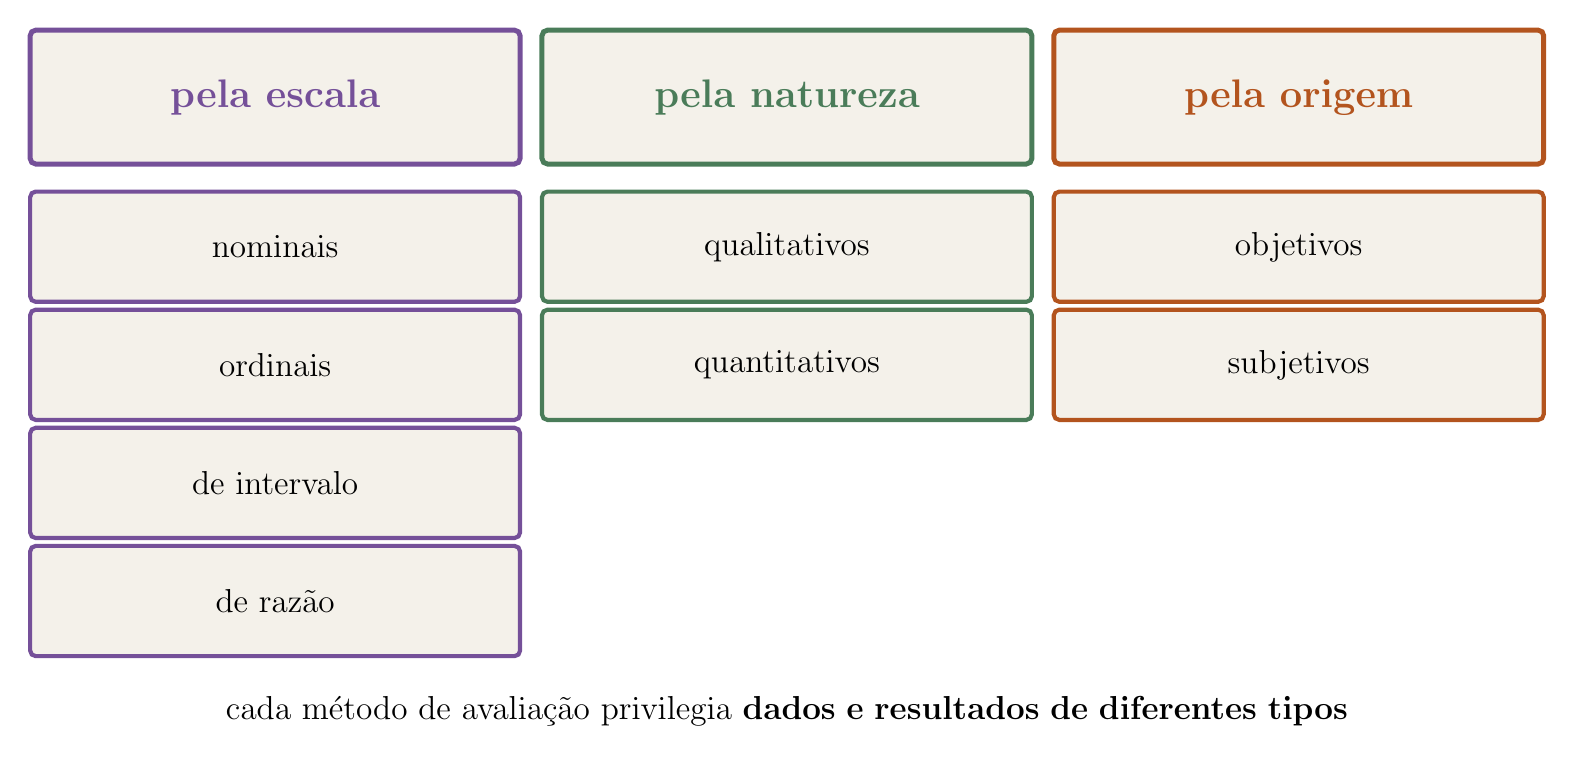
\begin{tikzpicture}[x=1cm,y=1cm]
\tikzset{h/.style={dbox, text width=5.8cm, minimum height=1.7cm, font=\Large\bfseries, line width=1.8pt},
        k/.style={dbox, text width=5.8cm, minimum height=1.4cm, font=\large, line width=1.5pt}}
\node[h, draw=dblue] at (3.2,6.8) {\textcolor{dblue}{pela escala}};
\node[k, draw=dblue] at (3.2,4.9) {nominais};
\node[k, draw=dblue] at (3.2,3.4) {ordinais};
\node[k, draw=dblue] at (3.2,1.9) {de intervalo};
\node[k, draw=dblue] at (3.2,0.4) {de razão};
\node[h, draw=dgreen] at (9.7,6.8) {\textcolor{dgreen}{pela natureza}};
\node[k, draw=dgreen] at (9.7,4.9) {qualitativos};
\node[k, draw=dgreen] at (9.7,3.4) {quantitativos};
\node[h, draw=dorange] at (16.2,6.8) {\textcolor{dorange}{pela origem}};
\node[k, draw=dorange] at (16.2,4.9) {objetivos};
\node[k, draw=dorange] at (16.2,3.4) {subjetivos};
\node[font=\large, text width=17cm, align=center] at (9.7,-1.0) {cada método de avaliação privilegia \textbf{dados e resultados de diferentes tipos}};
\end{tikzpicture}
\end{document}
